\documentclass[cs4size,a4paper]{ctexart}   
%==================== 数学符号公式 ============
\usepackage{amsmath}                 % AMS LaTeX宏包
\usepackage[style=1]{mdframed}
\usepackage{amsthm}
\usepackage{amsfonts}
\usepackage{mathrsfs}                % 英文花体字 体
\usepackage{bm}                      % 数学公式中的黑斜体
\usepackage{bbding,manfnt}           % 一些图标,如 \dbend
\usepackage{lettrine}                % 首字下沉,命令\lettrine
\def\attention{\lettrine[lines=2,lraise=0,nindent=0em]{\large\textdbend\hspace{1mm}}{}}
\usepackage{longtable}
\usepackage[toc,page]{appendix}
\usepackage{geometry}                % 页边距调整
\geometry{top=3.0cm,bottom=2.7cm,left=2.5cm,right=2.5cm}
%====================公式按章编号==========================
\numberwithin{equation}{section}
\numberwithin{table}{section}
\numberwithin{figure}{section}
%================= 基本格式预置 ===========================
\usepackage{fancyhdr}
\pagestyle{fancy}
\fancyhf{}  
\fancyfoot[C]{~\zihao{5} \thepage~}
\renewcommand{\headrulewidth}{0.65pt} 
\CTEXsetup[format={\centering\bfseries\zihao{-2}},name={第, 章}]{section}
\CTEXsetup[nameformat={\bfseries\zihao{3}}]{subsection}
\CTEXsetup[nameformat={\bfseries\zihao{4}}]{subsubsection}
%================== 图形支持宏包 =========================
\usepackage{subfigure}
\usepackage{graphicx}                % 嵌入png图像
\usepackage{color,xcolor}            % 支持彩色文本、底色、文本框等
\usepackage{hyperref}                % 交叉引用
\usepackage{caption}
\captionsetup{figurewithin=section}
%==================== 源码和流程图 =====================
\usepackage{listings}                % 粘贴源代码
\usepackage{xcolor}
\usepackage{color}
\definecolor{dkgreen}{rgb}{0,0.6,0}
\definecolor{gray}{rgb}{0.5,0.5,0.5}
\definecolor{mauve}{rgb}{0.58,0,0.82}
 \usepackage{xcolor}
 \lstset{
  %行号
    numbers=left,
    %背景框
    framexleftmargin=8mm,
    frame=none,
     %背景色
    %backgroundcolor=\color[rgb]{1,1,0.76},
     backgroundcolor=\color[RGB]{245,245,244},
     %样式
   keywordstyle=\bf\color{blue},
   identifierstyle=\bf,
    numberstyle=\color[RGB]{0,192,192},
    commentstyle=\it\color[RGB]{0,96,96},
   stringstyle=\rmfamily\slshape\color[RGB]{128,0,0},
   %显示空格
    showstringspaces=false
 }


%--------------------
\hypersetup{hidelinks}
\usepackage{booktabs}  
\usepackage{shorttoc}
\usepackage{tabu,tikz}
\usepackage{float}

\usepackage{multirow}



\tabcolsep=1ex
\tabulinesep=\tabcolsep
\newlength\tikzboxwidth
\newlength\tikzboxheight
\newcommand\tikzbox[1]{%
        \settowidth\tikzboxwidth{#1}%
        \settoheight\tikzboxheight{#1}%
        \begin{tikzpicture}
        \path[use as bounding box]
                (-0.5\tikzboxwidth,-0.5\tikzboxheight)rectangle
                (0.5\tikzboxwidth,0.5\tikzboxheight);
        \node[inner sep=\tabcolsep+0.5\arrayrulewidth,line width=0.5mm,draw=black]
                at(0,0){#1};
        \end{tikzpicture}%
        }

\makeatletter
\def\hlinew#1{%
  \noalign{\ifnum0=`}\fi\hrule \@height #1 \futurelet
   \reserved@a\@xhline}
   
\newcommand{\tabincell}[2]{\begin{tabular}{@{}#1@{}}#2\end{tabular}}%

\usepackage{subfigure}

\usepackage{CJK}
\usepackage{ifthen}


\usepackage{graphicx} 
\newcommand{\HRule}{\rule{\linewidth}{0.5mm}}

\newtheorem{Theorem}{定理}
\newtheorem{Lemma}{引理} 
%%使得公式随章节自动编号
\makeatletter
\@addtoreset{equation}{section}
\makeatother
\renewcommand{\theequation}{\arabic{section}.\arabic{equation}}

%-------------------------
	
\usepackage{pythonhighlight}
\usepackage{tikz}                    
\usepackage{tikz-3dplot}
\usetikzlibrary{shapes,arrows,positioning}

% 添加首行缩进,两个字符
\usepackage{indentfirst}
\setlength{\parindent}{2em}

% 参考文献标记
\usepackage[superscript]{cite}

% URL导入包
\usepackage{url}


%===================   正文开始    ===================
\begin{document}
%============== 封皮和前言 =================
\begin{titlepage}
	\begin{center}
		
\includegraphics[width=0.65\textwidth]{image/XJTU}\\[1cm]    
		\textsc{\LARGE 西安交通大学}\\[0.5cm]
		\textsc{\Large 计算机网络原理与应用课程作业}\\[0.5cm]
		\begin{tabular}{cc}%一个c表示有一列,格式为居中显示(center)
			姓名:&屈彬\\%第一行第一列和第二列  中间用&连接
			学号:&2140505062\\%第二行第一列和第二列  中间用&连接
			次数:&第1次\\
			日期:&\today\\
		\end{tabular}
	\end{center}
\end{titlepage}
\pagestyle{plain}
\pagenumbering{arabic}
%============== 正文   =================
\pagestyle{fancy}
\begin{center}
	\large{利用Wireshark软件获取并分析TLS协议}\\
\end{center}
\begin{flushleft}
	\tableofcontents
	\section{实验背景}
		\subsection{TLS简介}
			\qquad 
TLS全称“Transport Layer Security(安全传输层)”,用于在两个通信应用程序之间提供保密性和数据完整性,常用于Web应用中客户端与服务器的加密通信。虽然TLS协议被定义为传输层的安全协议,但实际在抓包结果中可以看到TLS协议部分是被封装在TCP等传输层协议内的,而应用层的内容则封装在TLS内。在登录西安交通大学学生版统一认证网关的过程中,客户端页面也采用TLS加密方式向服务器提交表单,因此通过本实验也能对西安交通大学统一认证网关的安全机制有更好的了解。\\
\qquad
通过查阅国内相关文献 \cite{TLS-1} 以及国外的一些文献 \cite{TLS-2} ,可以了解到TLS协议由记录协议、更改密码协议以及警告协议三个高层协议构成,其中,记录协议还包括握手子协议。记录协议从高层ssL子协议收到数据后,对它们进行数据分段、压缩、认证和加密形成ssL记录;更改密码规格协议将密文状态由挂起状态复制到当前状态;警告协议用来传递ssL的相关警告。由于握手过程是可以被Wireshark软件轻易捕获的,在抓包时,我们主要关心的是TLS协议中的握手过程。TLS的握手过程如图 \ref{fig1} 所示。\\
\begin{figure}
	\centering
	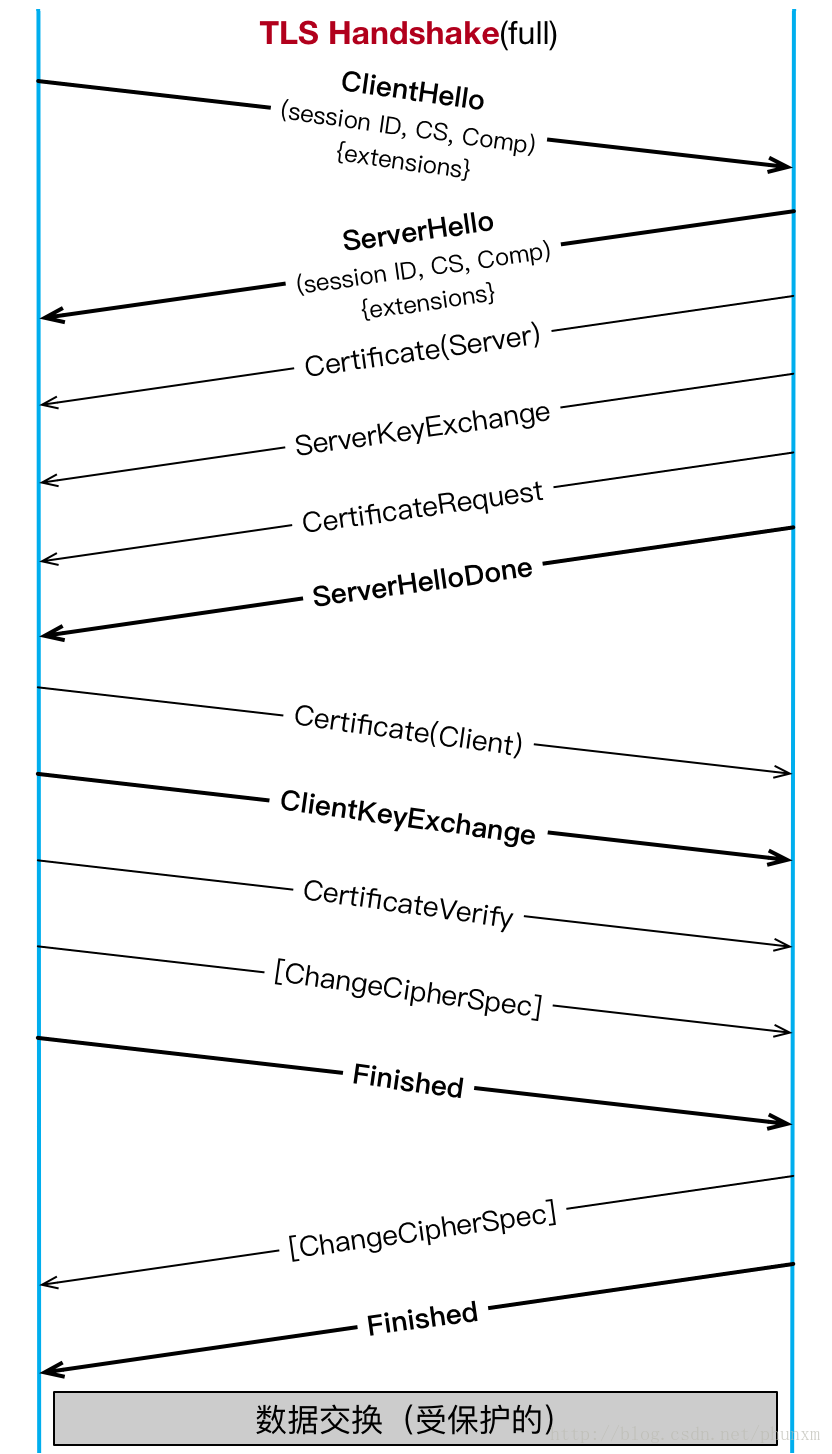
\includegraphics[width=8cm]{image/TLS-Handshake}
	\caption{TLS协议握手过程 \cite{TLS-3}}
	\label{fig1}
\end{figure}
\qquad
在图 \ref{fig1} 中,左侧代表客户端,右侧代表服务端。当客户端向服务端发起握手时,客户端首先向服务端发送“ClientHello”字段,包含会话ID(Session ID)等信息;服务端收到“ClientHello”字段后,返回一个“ServerHello”字段,同样包含会话ID等信息;之后服务端和客户端之间会进行密钥交换,在结束握手前,客户端和服务器还向依次向对方发送更改密钥的信息。\\
\qquad
但在实际的网络应用中,TLS协议的握手过程是否真的如图 \ref{fig1} 所示。本实验将通过Wireshark软件对西安交通大学学生版统一身份认证网关的登录过程进行抓包分析,以探究竟。\\
		\subsection{实验目标}
			\begin{enumerate}
	\item 利用Wireshark软件对西安交通大学学生版统一认证网关的登录过程进行抓包。
	\item 分析不同层的重要协议头字段。
	\item 分析TLS协议中记录协议与其子协议的关系。
	\item 理解和分析TLS协议的握手过程。
	\item 说明TLS协议握手过程体现了计算机网络的何种概念和原理。
	\item 解密客户端向服务端提交的表单。
\end{enumerate}
	\section{实验工具}
		\begin{enumerate}
	\item Wireshark软件:用于获取网络通信过程经过本地的数据包。本实验所使用的版本为2.4.5。
	\item 支持IE6以上内核的浏览器:用于访问西安交通大学学生版统一身份认证网关。
	\item CTeX + TeXstudio:用于报告写作(首次使用)。
\end{enumerate}
	\section{实验过程}
		\subsection{抓包过程}
			\qquad
首先确保网络通畅,查看本机IPv4地址(调用Windows控制台ipconfig命令查看)和服务端IPv4地址(打开相应的网页,按F12查看),本实验中客户端地址为192.168.123.64,客户端处于一个子网中,服务端地址为202.117.1.185。\\
\qquad
在浏览器URL栏输入“https://cas.xjtu.edu.cn/login”,回车后打开西安交通大学学生版统一身份认证网关,如图 \ref{fig2} 所示。\\
\begin{figure}
	\centering
	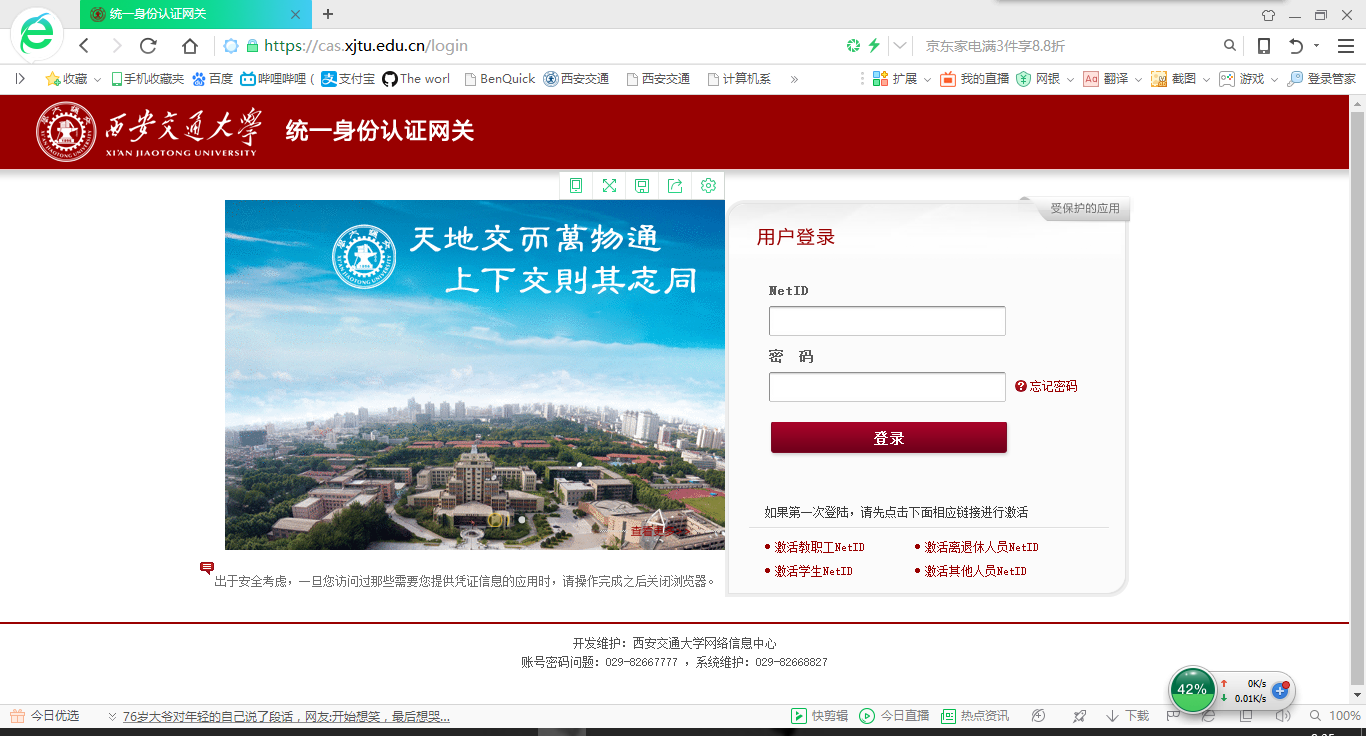
\includegraphics[width=12cm]{image/XJTU-Certificate}
	\caption{西安交通大学学生版统一身份认证网关}
	\label{fig2}
\end{figure}
\qquad
打开Wireshark软件,在初始界面选择活跃的网络连接,如图 \ref{fig3} 所示。本实验中客户端计算机通过无线局域网上网,所以选择WLAN连接。\\
\begin{figure}
	\centering
	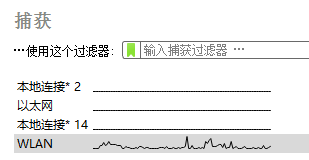
\includegraphics[width=8cm]{image/Wireshark-1}
	\caption{在Wireshark初始界面选择活跃的网络连接}
	\label{fig3}
\end{figure}
\qquad
在打开验证页面上输入用户名和密码,在点击登录之前,先确定Wireshark开始捕获分组,然后再进行登录。当页面上提示登陆成功后,停止捕获分组。将捕获到的分组保存为本地文件,以方便日后查看。本次实验中捕获到的分组如图 \ref{fig4} 所示。\\
\begin{figure}
	\centering
	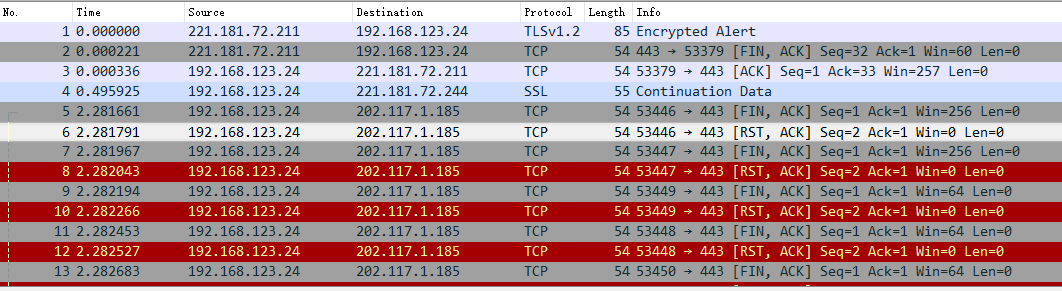
\includegraphics[width=12cm]{image/Wireshark-2}
	\caption{Wireshark捕获的分组(局部)}
	\label{fig4}
\end{figure}
\qquad
在图 \ref{fig4} 中,不同类型的分组用不同的颜色标出,可以通过点击“视图->着色规则”菜单项查看不同颜色所代表的的分组类型,如图 \ref{fig5} 所示。根据图 \ref{fig5} ,可以看到图 \ref{fig4} 捕获的分组中既包括UDP分组、TCP分组、TCP握手分组和TCP RST(复位)分组。其中,客户端(192.168.123.64)在与认证网关服务端(202.117.1.185)建立连接的过程中有多个RST分组(红色);产生RST的原因很多,不过根据图 \ref{fig4} 捕获的分组来看是由于服务端的443端口未被进程监听或被占用,而客户端又向服务端发送目标端口为443的连接请求,这时客户端则会发送RST分组以重新建立连接。\\
\begin{figure}
	\centering
	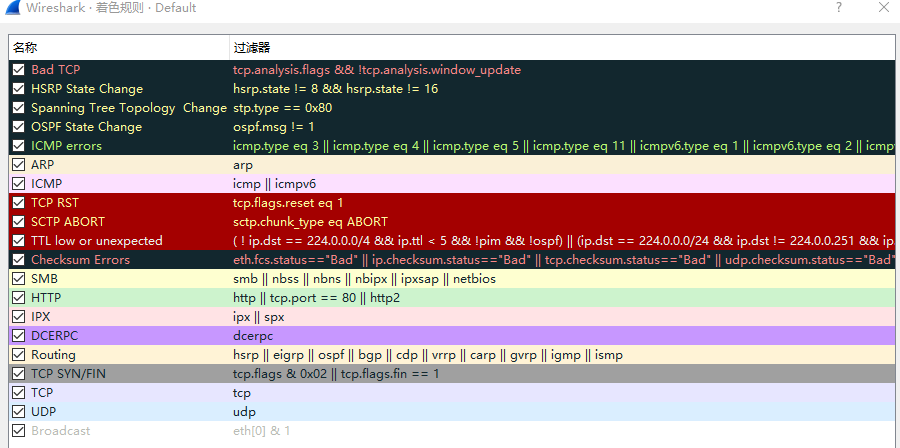
\includegraphics[width=12cm]{image/Wireshark-3}
	\caption{着色规则}
	\label{fig5}
\end{figure}
		\subsection{TLS握手过程分析}
			\qquad
在过滤栏上输入“ip.addr == 202.117.1.185”过滤掉与认证登录过程不相关的分组,最后确定与TLS协议握手过程相关的分组为第141号分组到第147号分组,如图 \ref{fig6} 所示。点击141号(Client Hello)分组,可以看到该分组中不同网络层的重要字段信息,如图 \ref{fig7} 所示。\\
\begin{figure}
	\centering
	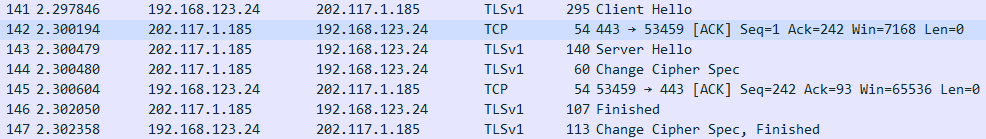
\includegraphics[width=12cm]{image/TLS-1}
	\caption{与TLS握手过程相关的分组}
	\label{fig6}
\end{figure}
\begin{figure}
	\centering
	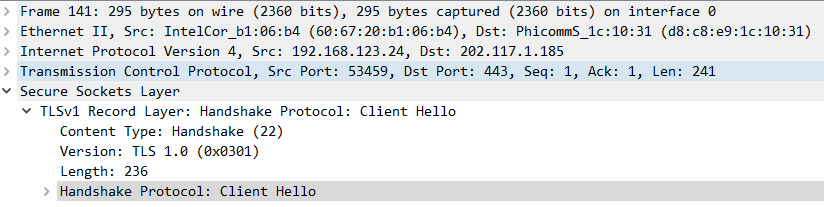
\includegraphics[width=12cm]{image/layer-1}
	\caption{Client Hello分组中不同层次的重要字段}
	\label{fig7}
\end{figure}
\qquad
根据图 \ref{fig7} 反映的分组字段信息,可见最上方的物理层字段反映了分组帧长度为295个字节。被物理层封装的数据链路层,协议为“Ethernet II(第二代以太网)”,显示客户端的设备为“Intel Core(英特尔酷睿系列核心)”,MAC地址为60:67:20:b1:06:b4(十六进制格式);服务端的设备为phi卡,MAC地址为d8:c8:e9:1c:10:31。被数据链路层封装的网络层,协议为IPv4,源地址为192.168.123.24,目标地址为202.117.1.185。被网络层封装的传输层,协议为TCP,源端口为53459,目标端口为443,分组序号(Seq)为1,应答序号(Ack)为1,分组长度为241个字节。重点的SSL(安全传输层)被封装在TCP层中,协议为TLSv1,其中又封装了长度为236个字节的TLS记录层,TLS记录层中又封装了TLS握手协议层,而该握手协议层的握手信息为“Client Hello”。该分组逐层封装的过程体现了计算机网络中的分层思想,将一个分组按类型分为不同的层次有利于逐层分析,简化网络模型。\\
\qquad
和握手协议一样,TLS协议中的更改密码协议也是封装在记录协议中的,通过点击144号分组可以发现这一点,如图 \ref{fig8} 所示。通过观察其他TLS分组的协议结构,验证了记录协议与握手协议、更改密码协议、应用数据协议等其他子协议的层次关系,即这些子协议都封装在记录协议中。\\
\begin{figure}
	\centering
	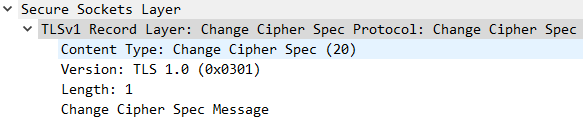
\includegraphics[width=12cm]{image/layer-2}
	\caption{Change Cipher Spec分组中TLS协议层}
	\label{fig8}
\end{figure}
\qquad
根据图 \ref{fig6} 以及各个分组的分层字段信息,可以归纳出本实验中TLS协议握手过程如图 \ref{fig9} 所示。根据图 \ref{fig9} ,TLS协议的握手过程可分为以下步骤:\\
\begin{enumerate}
	\item 客户端向服务端发送Client Hello分组,这组分组包含一段会话编号(Session ID)以及一段随机密钥(如图 \ref{fig10}所示,这是客户端的私钥),期望建立TLS连接,开辟临时会话。
	\item 服务端回复一段TCP应答分组,作为对客户端上一个TCP分组的应答。
	\item 服务端向客户端发送Server Hello分组,这组分组包含一段与Client Hello分组中一致的会话编号(Session ID)和一段随机密钥(如图 \ref{fig11}所示,服务端使用客户端之前发送的私钥给自己的随机密钥加密,这段密钥正是服务端加密后的给客户端共用的公钥),表示同意建立TLS连接,并且接着Server Hello分组的Change Cipher Spec分组中通知客户端使用服务端提供的公钥加密。
	\item 客户端对服务端上一个TCP分组进行应答。
	\item 服务端收到客户端应答后,确认客户端已经知道要使用约定好的公钥加密和解密数据,发送Finished分组期望结束握手。
	\item 客户端收到结束握手分组后,发送Change Cipher Spec分组和Finished分组,表明已完成密钥的更改,结束握手。
\end{enumerate}
\begin{figure}
	\centering
	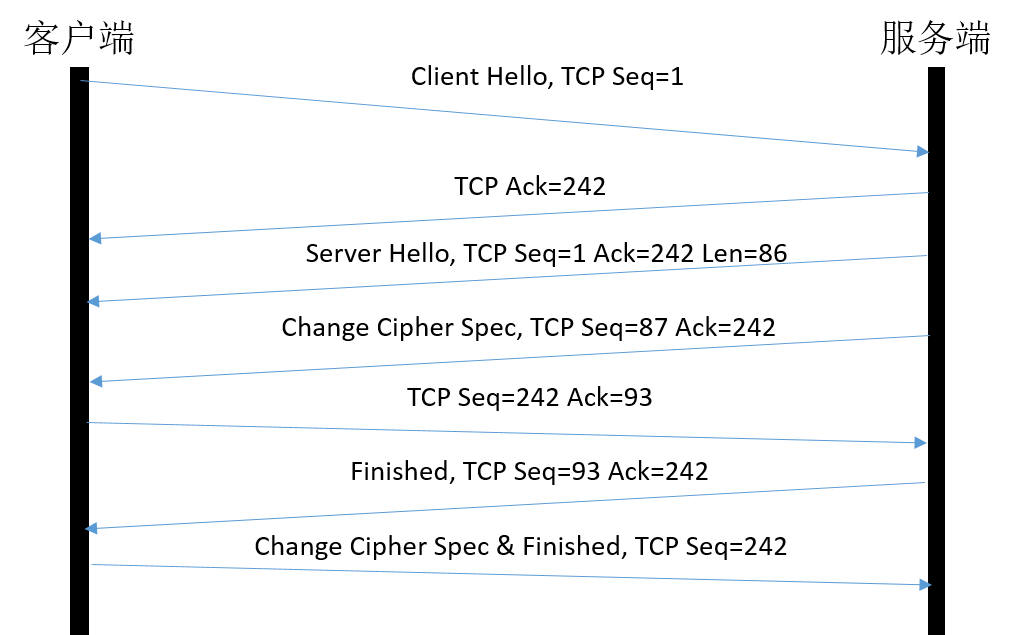
\includegraphics[width=12cm]{image/TLS-Handshake-1}
	\caption{本实验中TLS协议握手过程}
	\label{fig9}
\end{figure}
\begin{figure}
	\centering
	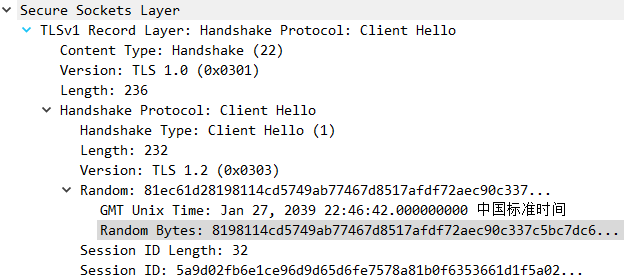
\includegraphics[width=12cm]{image/TLS-Handshake-2}
	\caption{Client Hello分组TLS协议部分}
	\label{fig10}
\end{figure}
\begin{figure}
	\centering
	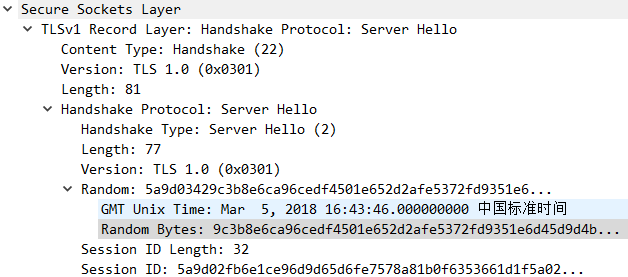
\includegraphics[width=12cm]{image/TLS-Handshake-3}
	\caption{Server Hello分组TLS协议部分}
	\label{fig11}
\end{figure}
\qquad
完成TLS握手后,客户端与服务端的临时会话便使用来自服务端的相同的密钥进行数据的加密和解密,本次临时会话结束后,TLS连接关闭,本次临时会话的密钥无法用于下次会话。以上TLS协议的握手过程说明TLS协议采用面向连接的服务,对应用数据采用对称加密技术。
		\subsection{表单解密}
			\qquad
为了充分验证本次实验中Wireshark软件真的抓到了登录过程中客户端向服务端提交的表单,下面将对捕获到的分组中TLS协议应用数据层的内容进行解密,以得到表单明文。完成解密后的分组如图 \ref{fig12} 所示。其中,标记为绿色,协议为HTTP的分组正是解密后的TLS应用数据层内容。\\
\begin{figure}
	\centering
	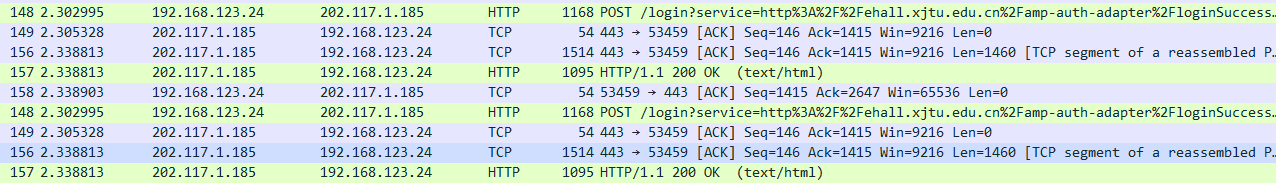
\includegraphics[width=12cm]{image/http-1}
	\caption{解密后分组(局部)}
	\label{fig12}
\end{figure}
\qquad
在解密之前,TLS应用数据层的内容是加密后的乱码,无法看到明文。通过上一小节对TLS握手过程的分析,得知这些内容是使用服务端提供的公钥加密的,因此客户端上应该保存有这份公钥,只要拿到这份公钥就可以对内容进行解密。事实上,一般的浏览器都会将TLS握手后得到的公钥保存在本地,通过设置环境变量可以改变公钥存放的位置,如图 \ref{fig13} 所示。然后在Wireshark菜单栏中依次点击“编辑->首选项->Protocol->SSL”,在出现的窗口中找到“(Pre)-Master-Secret log filename”下方的文本框,输入公钥保存的位置,如图 \ref{fig14} 所示。\\
\qquad
完成以上设置后再开始抓包。得到分组后,右键点击需要解密的分组,在弹出的菜单中点击“解码为...”,根据分组字段内容设置好相应的参数后即可完成解密。本实验中最终解密得到的客户端向服务端提交的登录表单的内容如图 \ref{fig15} 所示,表单中包含用户名、密码等信息。
\begin{figure}
	\centering
	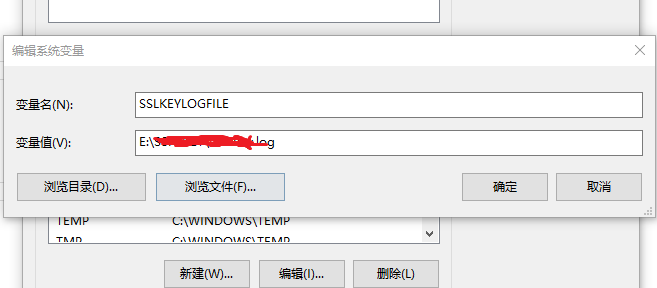
\includegraphics[width=12cm]{image/SSHKEY}
	\caption{通过设置环境变量改变浏览器保存公钥的位置}
	\label{fig13}
\end{figure}
\begin{figure}
	\centering
	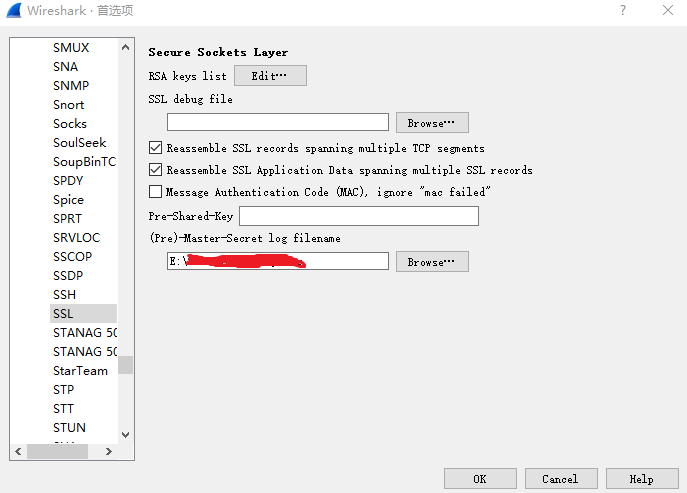
\includegraphics[width=12cm]{image/SSHKEY-1}
	\caption{在Wireshark中设置公钥保存位置}
	\label{fig14}
\end{figure}
\begin{figure}
	\centering
	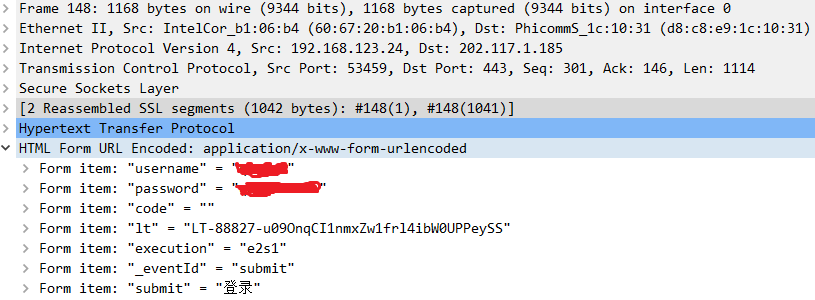
\includegraphics[width=12cm]{image/SSHKEY-2}
	\caption{解密后登录表单的内容}
	\label{fig15}
\end{figure}
	\section{实验结论}
	
\end{flushleft}
    
%============= 参考文献 =====================
\bibliographystyle{unsrt}
%\%\include{body/acknowledge}
%addcontentsline{toc}{section}{参考文献}
\bibliography{bib/bibfile}
%\clearpage
%=============  致谢  ======================
%\include{body/appendices}

\end{document}
%%%%%%%%%% 结束 %%%%%%%%%%